
\section{Validación}

En esta sección se estudia el mismo perfil NACA sin deflexión de flaps. Primeramente se calcula la pendiente de sustentación $\left( C_{l\alpha} \right)$, el ángulo de sustentación nula $\left( \alpha_{l0} \right)$ y el coeficiente de momento en el centro aerodinámico $\left( C_{m0} \right)$. Posteriormente, se calcula la eficiencia del flap para distintos \emph{flap-chord ratios} y se verifica la efectividad de la corrección de flap.

Numéricamente se obtienen el $C_l$ y el $C_{m0}$ para un amplio rango de ángulos de ataque $\left( -30 \degrees \text{ a } 30 \degrees \right)$, con $N = 200$ paneles. Se elige un tramo lineal de $\pm 10\degrees$ y se calcula el $C_{l\alpha}$ como la pendiente de la recta de sustentación. El $\alpha_{l0}$ se obtiene con el método de la bisección y el $C_{m0}$ se calcula como el promedio en el rango lineal elegido. La variación máxima de $C_{m0}$ es de $3.53\%$, por lo que se considera constante.

La curva de sustentación en el tramo lineal obtenida es:
\begin{equation}
    C_l = 0.1091 \alpha - 0.2254 \quad
    \left[ \alpha \right] = \mathrm{deg}
\end{equation}

En la figura \ref{fig:validacion_abbot_Cl} se muestra el $C_l$ experimental, con y sin flap, en función de $\alpha$, para el perfil NACA 2408. Se recogen curvas para distintos números de Reynolds $\left( \reynolds \right)$. Se toma como referencia la curva de $\reynolds = 9 \cdot 10^6$. Para obtener $C_{l\alpha}$ y $\alpha_{l0}$ experimentales se escogen dos puntos representativos del régimen lineal: $\alpha_1 = -8\degrees$, $C_{l1} = -0.6$ y $\alpha_2 = 4\degrees$, $C_{l2} = 0.6$. 

\begin{figure}[ht] 
    \centering
    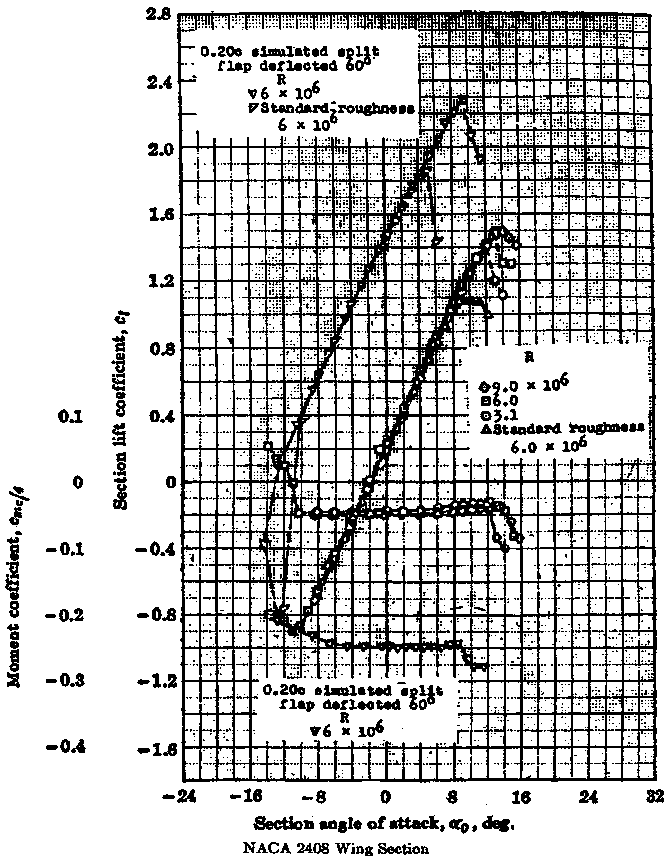
\includegraphics[width=\linewidth]{imagenes/validacion/validacion_abbot_Cl.pdf}
    \caption{Curva de sustentación $\left( C_l(\alpha) \right)$ en función del ángulo de ataque $\left( \alpha \right)$, con y sin flap de borde de salida, para distintos números de Reynolds $\left( \reynolds \right)$. A partir de \cite{abbott}.}
    \label{fig:validacion_abbot_Cl}
\end{figure}

En la figura \ref{fig:validacion_abbot_Cm0} se muestran el coeficiente de resistencia aerodinámica $\left( C_d \right)$ y el $C_{m0}$ en función de $\alpha$. En el rango de $C_l$ usado anteriormente, $C_{m0}$ es ligeramente superior a $-0.05$. A falta de mayor precisión, se elige $C_{m0} = -0.05$.

\begin{figure}[ht] 
    \centering

    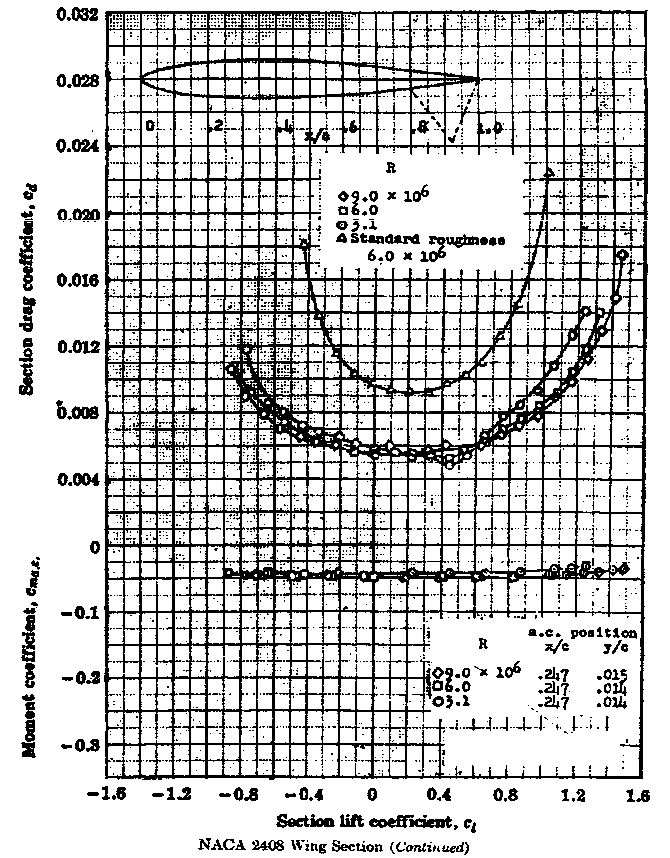
\includegraphics[width=\linewidth]{imagenes/validacion/validacion_abbot_Cm0.pdf}
    \caption{Coeficiente de resistencia aerodinámica $\left( C_d \right)$ y coeficiente de momento libre $\left( C_{m0} \right)$, en función del coeficiente de sustentación $\left( C_l \right)$, para distintos números de Reynolds $\left( \reynolds \right)$. A partir de \cite{abbott}.}
    \label{fig:validacion_abbot_Cm0}
\end{figure}

En la tabla \ref{tab:comparacion_numerico_experimental_error} se recogen los valores obtenidos mediante el DVM y los experimentales, con los correspondientes errores.

\begin{table}[h]
    \centering
    \begin{tabular}{lrrr}
        \toprule[0.5mm]
        Variable & Numérico & Experimental & Error $\left( \% \right)$ \\
        \midrule[0.25mm]
        $C_{l\alpha} \ \left( 1 /\mathrm{deg} \right)$ & 
        $0.1091$ & $0.1000$ & $9.12 \%$ \\
        $\alpha_{l0} \ \left( \mathrm{deg} \right)$ & $-2.0654$ & 
        $-2.0000$ & $-3.27 \%$ \\
        $C_{m0}$ & $-0.0527$ & $-0.0500$ & $-5.40\%$ \\
        \bottomrule[0.5mm]
    \end{tabular}
    \caption{Resultados numéricos mediante DVM, experimentales y error relativo, para $C_{l\alpha}$, $\alpha_{l0}$ y $C_{m0}$. Resultados experimentales a partir de \cite{abbott}.}
    \label{tab:comparacion_numerico_experimental_error}
\end{table}

Como se observa en la tabla \ref{tab:comparacion_numerico_experimental_error}, el error relativo máximo es inferior al $10\%$. Por consiguiente, los resultados numéricos obtenidos con el DVM son cercanos a los experimentales dados por Abbott \& Doenhoff (1959). Considerando que cualquier medida experimental conlleva cierto error, se concluye que el error es menospreciable.

Para validar los parámetros aerodinámicos del perfil NACA 2408 con flap de borde de salida, se comparan los calculados empleando el DVM con los dados por Abbott \& Doenhoff.

Seguidamente, se estudia el factor de eficiencia del flap $\left( \partial \alpha_{l0} / \partial \eta \right)$ en función del \emph{flap-chord ratio} $\left( E \right)$. Este último se define como $E = 1 - x_h/c$, donde $c$ es la cuerda y $x_h$ es la posición del eje de charnela respecto $c$. 

La eficiencia del flap de borde de salida se define como la variación del ángulo de sustentación nula respecto del ángulo de deflexión del flap $\left( \eta \right)$ \cite{ortega},
\begin{equation}
    \frac{\partial \alpha_{l0}}{\partial \eta} = 
    - \left( 1 - \frac{\theta_h}{\pi} + \frac{\sin{\theta_h}}{\pi} \right)
\end{equation}
La variación en el ángulo de sustentación nula se calcula como
\begin{equation}
    \Delta \alpha_{l0} = \frac{\partial \alpha_{l0}}{\partial \eta} \eta
\end{equation}
Según la TAT la pendiente de sustentación $C_{l\alpha}$ no varía con la deflexión de flap \cite{ortega}. Conocidos los coeficientes de sustentación para un ángulo de ataque, sin deflexión de flap $\left( C_l \right)$ y con deflexión de flap $\left( C_{l,f} \right)$ de ángulo $\eta$, el factor de eficiencia del flap se determina a partir de 
\begin{equation} \label{eq:calculo_factor_eficiencia}
    \frac{\partial \alpha_{l0}}{\partial \eta} = 
    \frac{C_l - C_{l,f}}{C_{l\alpha} \eta}
\end{equation}
De \eqref{eq:calculo_factor_eficiencia} se aprecia que el factor de eficiencia es negativo, pues $C_{l,f} > C_l$ para deflexiones de flap positivas.

Para obtener el factor de eficiencia del flap se elige un ángulo de ataque $\alpha = 0$ y un ángulo de deflexión del flap $\eta = 10\degrees$. Posteriormente se calcula $C_{l,f}$ con $N = 200$ paneles. Conocidos $C_l$ y $C_{l\alpha}$, se aplica \eqref{eq:calculo_factor_eficiencia}. Para el cálculo del factor de eficiencia corregido, se aplica un factor de corrección de $0.8$, correspondiente a flap simple con deflexión $\eta = 10\degrees$ según \cite{mccormick_flap}.

El factor de eficiencia experimental para \emph{flap-chord ratio} en el rango $0$--$0.5$ dado por Abbott \& Doenhoff se muestra en la figura \ref{fig:validacion_abbot_flap}.

\begin{figure}[ht] 
    \centering
    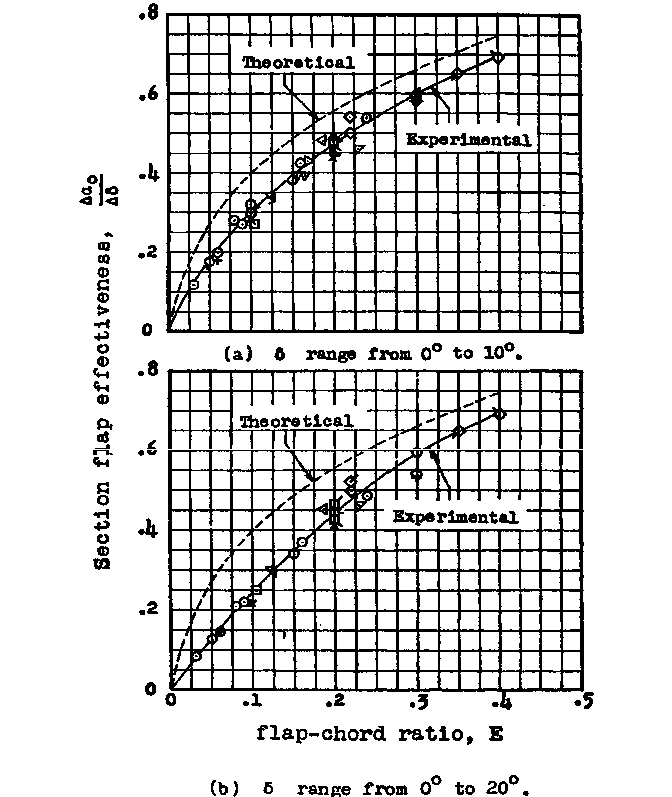
\includegraphics[width=\linewidth]{imagenes/validacion/validacion_abbot_flap.pdf}
    \caption{Factores de eficiencia del flap $\left( \partial \alpha_{l0} / \partial \eta \right)$ teórico y experimental, en función del \emph{flap-chord ratio} $\left( E \right)$ según Abbott \& Doenhoff. A partir de \cite{abbott_flap}.}
    \label{fig:validacion_abbot_flap}
\end{figure}

En la figura \ref{fig:validacion_flap} se representa el factor de eficiencia según DVM, el factor corregido y el experimental, para \emph{flap-chord ratio} en el rango $0$--$0.40$. Como se ha comentado, para $\eta > 0$, el factor de eficiencia es negativo. Por consiguiente, realmente se representa el valor absoluto del factor. En la tabla \ref{tab:validacion_flap} se recogen los factores de eficiencia del flap y los errores relativos respecto del valor experimental.

\begin{figure}[ht] 
    \centering
    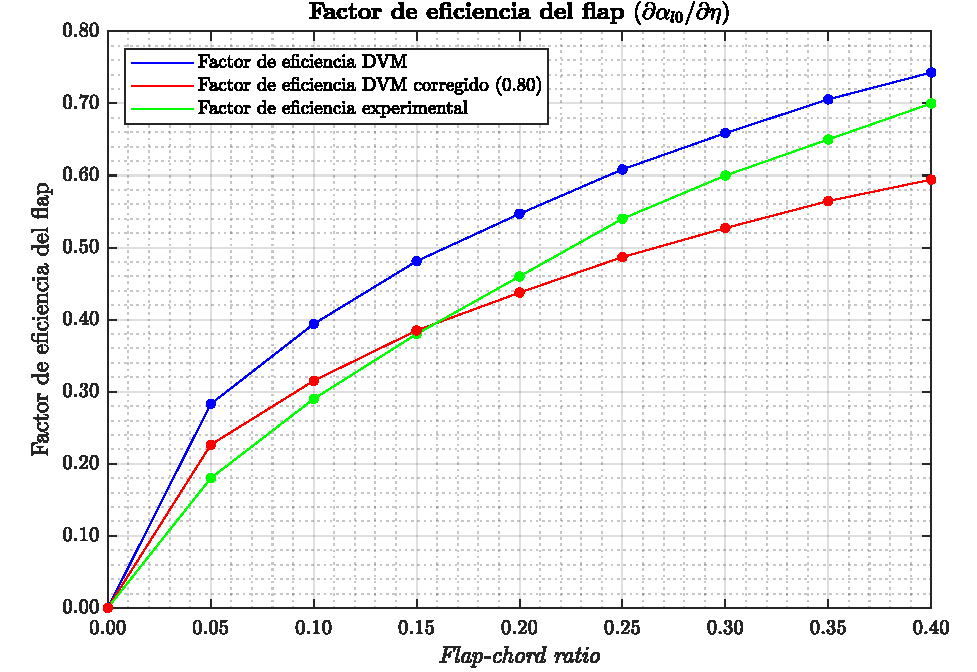
\includegraphics[width=\linewidth]{imagenes/validacion/validacion_flap.pdf}
    \caption{Factor de eficiencia del flap $\left( \partial \alpha_{l0} / \partial \eta \right)$ según DVM, corregido (factor $0.8$) y experimental en función del \emph{flap-chord ratio} $\left( E \right)$. Ángulo de ataque $\alpha = 0$, ángulo de deflexión del flap $\eta = 10\degrees$.}
    \label{fig:validacion_flap}
\end{figure}

Se observa que el factor de eficiencia del flap aumenta con $E$. El efecto que introduce la combadura positiva sobre un perfil es un ángulo de sustentación nula negativo, \ie, $\alpha_{l0} < 0$. Cuanto mayor es la combadura, menor es $\alpha_{l0}$. Para una misma deflexión de flap $\eta$, a medida que aumenta $E$, también aumenta la combadura, reduciendo aún más $\alpha_{l0}$. Por consiguiente, el factor de eficiencia del flap debe aumentar.

Se observa gran similitud entre los valores del DVM corregido y los experimentales para $E \leq 0.30$. A medida que $E$ crece, la diferencia entre ambas curvas aumenta. En la región anterior al borde de salida la capa límite tiene un espesor considerable. Ello implica que el flap actúe sobre un flujo de menor energía. En estas condiciones, el alcance de la TAT es limitado. Por consiguiente, para $E$ pequeñas el factor de eficiencia es considerablemente superior al experimental, por lo que es necesario introducir el factor de corrección. A medida que $E$ aumenta, la similitud entre ambos es mayor, pues el flap actúa sobre un flujo más energético.

\begin{table}[h]
    \centering
    \begin{tabular}{llllll}
        \toprule[0.5mm]
        & & & & \multicolumn{2}{c}{Error $\left( \% \right)$} \\
        \cline{5-6} \rule{0pt}{2ex}
        \makecell[l]{$E$} & DVM & Corr. & Exp. & DVM & Corr. \\
        \midrule[0.25mm]
        $ 0.00$  &  $    0.00$  &  $     0.00$  &  $    0.00$  &  $    0.00$  &  $    0.00$	\\
        $ 0.05$  &  $    0.28$  &  $    0.23$  &  $    0.18$  &  $   57.23$  &  $   25.78$	\\
        $ 0.10$  &  $    0.39$  &  $    0.32$  &  $    0.29$  &  $   35.85$  &  $    8.68$	\\
        $ 0.15$  &  $    0.48$  &  $    0.38$  &  $    0.38$  &  $   26.63$  &  $    1.30$	\\
        $ 0.20$  &  $    0.55$  &  $    0.44$  &  $    0.46$  &  $   18.89$  &  $    4.89$	\\
        $ 0.25$  &  $    0.61$  &  $    0.49$  &  $    0.54$  &  $   12.69$  &  $    9.85$	\\
        $ 0.30$  &  $    0.66$  &  $    0.53$  &  $    0.60$  &  $    9.81$  &  $   12.15$	\\
        $ 0.35$  &  $    0.71$  &  $    0.56$  &  $    0.65$  &  $    8.57$  &  $   13.15$	\\
        $ 0.40$  &  $    0.74$  &  $    0.59$  &  $    0.70$  &  $    6.13$  &  $   15.10$	\\
        \bottomrule[0.5mm]
    \end{tabular}
    \caption{Factor de eficiencia del flap $\left( \partial \alpha_{l0} / \partial \eta \right)$ según DVM, corregido (factor $0.8$), experimental y errores relativos en función del \emph{flap-chord ratio} $\left( E \right)$. Ángulo de ataque $\alpha = 0$, ángulo de deflexión del flap $\eta = 10\degrees$.}
    \label{tab:validacion_flap}
\end{table}








